
\newpage
\section{Objetivos}
\label{sec:target}

\justifying \setlength{\parindent}{1.27cm}
\normalsize\mdseries

El proyecto toma base en la siguiente arquitectura:

%   Descripción de la figura
\begin{figure}[h]
    \centering
    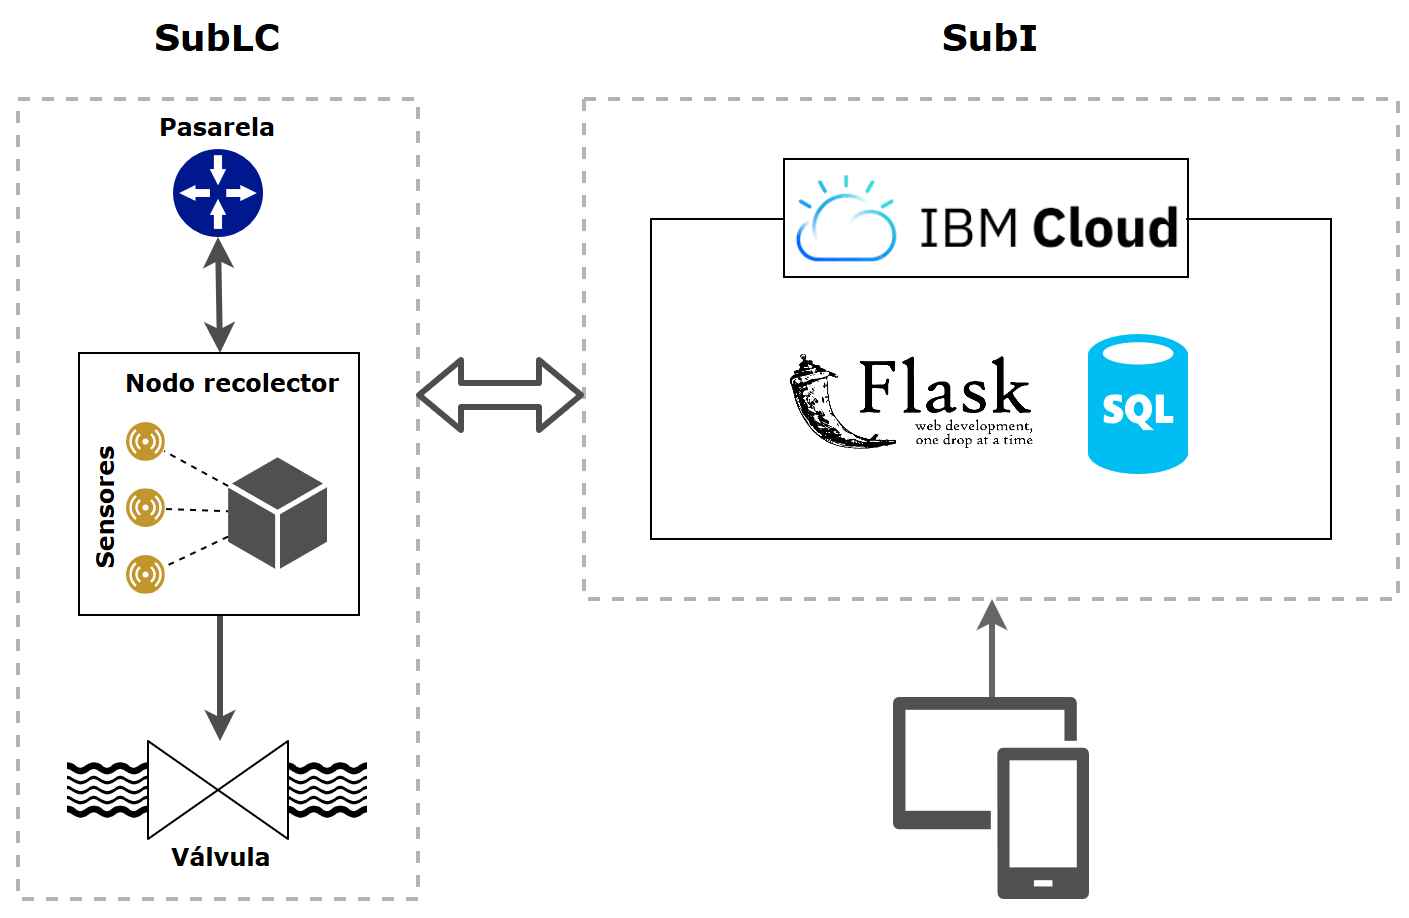
\includegraphics[scale=0.5]{figures/diagrams/architecture.png}
    \caption{Arquitectura del sistema.}
    \label{fig:architecture}
\end{figure}

En la figura \ref{fig:architecture} podemos ver cómo, el usuario, desde cualquier dispositivo accedería a un servicio \textit{cloud} y así conectar y/o controlar el sistema. Como ya se ha mencionado previamente, y reflejado en la propia ilustración, vemos los dos subsistemas del proyecto, los cuales se describirán a continuación:

\begin{description}
    \item [\textbf{SubLC}] Éste es el núcleo del proyecto. Se compone de 3 elementos fundamentales:
    \begin{itemize}
        \item Nodo recolector: Controlador con acceso a datos del entorno proporcionados por sensores.
        \item Válvula: Sistema de control del caudal de agua de una específica sección del terreno. Debe ser eléctricamente manejable para poder ajustar su medida (electroválvula).
        \item Pasarela: Controlador que, como su propio nombre indica, actúa de pasarela entre los nodos recolectores y el subsistema SubI.
    \end{itemize}
    \item [\textbf{SubI}] Controla al subsistema SubLC y actúa como interfaz entre éste y el usuario. Además tiene la tarea de almacenar y analizar los datos recogidos. Se encontraría alojado en la nube.
\end{description}